% Author: Dun-Ming Huang
% Email: dunmingbrandonhuang@berkeley.edu
% CSM16A Fall 2022
\qns{Get Rotated}

\textbf{Learning Goals}: \\
Learn how to \textbf{apply matrix transformations} and practice \textbf{designing algorithms for related operations}. \\
This question is built off the prior assignments and discussions of EECS 16A in Fall 2022 regarding rotation matrices.

\meta{
    Before starting with this question, here are a few advises for mentors:
    \begin{itemize}
        \item You \textbf{definitely want to solve this question on your own before teaching}. The solutions can take a lot of effort to explain.
        \item When explaining solutions, it really \textbf{helps to graph} rotations and translations out.
        \item To prevent common misunderstanding: \textbf{translation is not a linear transformation}. Matrix multiplications are linear transformations, but translations are matrix additions.
    \end{itemize}
}

\textit{Review: a pre-image is the figure before transformation, and an image is the figure after the transformation.} \\
Wanting to impress your lab partner who knows everything transforming points, you responded so: \\
"You know the rules, and so do I".
Your partner decided to give you a quiz on matrix transformations in return:

\begin{enumerate}
    \item {
        We learned in lecture that the rotation matrix for rotating a point $(x, y)$ into $(x', y')$ around the origin, by angle ${\theta}$ is:
        \[
            \begin{bmatrix} x' \\ y' \end{bmatrix} = 
            \begin{bmatrix}
                cos(\theta) & -sin(\theta) \\
                sin(\theta) & cos(\theta)
            \end{bmatrix}
            \begin{bmatrix} x \\ y \end{bmatrix}
        \]
        Try to derive it. \\
        \textit{(Hint: try \textbf{drawing the vectors} $\begin{bmatrix} x & y \end{bmatrix}^T$ and $\begin{bmatrix} x' & y' \end{bmatrix}^T$ out, \textbf{and the angles between those vectors}.)}
        
    }
    \meta {
        \begin{itemize}
            \item To lead students on the derivation process, mentors can also graph Figure 0.1 (in the solution) on the board before hand.
            \item Mentors can also provide the summation of angle formula on the way.
        \end{itemize}
        
    }
    \ans{
        Since we are \textbf{rotating using the origin as the center of rotation}, we would \textbf{graph the angle of rotation with its vertex at the origin}. \\
        %\begin{ln-fig}{The Rotation of a Point}{}
            \begin{center}
                % Author: Dun-Ming Huang
% Email: dunmingbrandonhuang@berkeley.edu
% CSM16A Fall 2022
%Code references advises on https://tex.stackexchange.com/questions/256863/drawing-and-labeling-angles-in-an-axis-environment

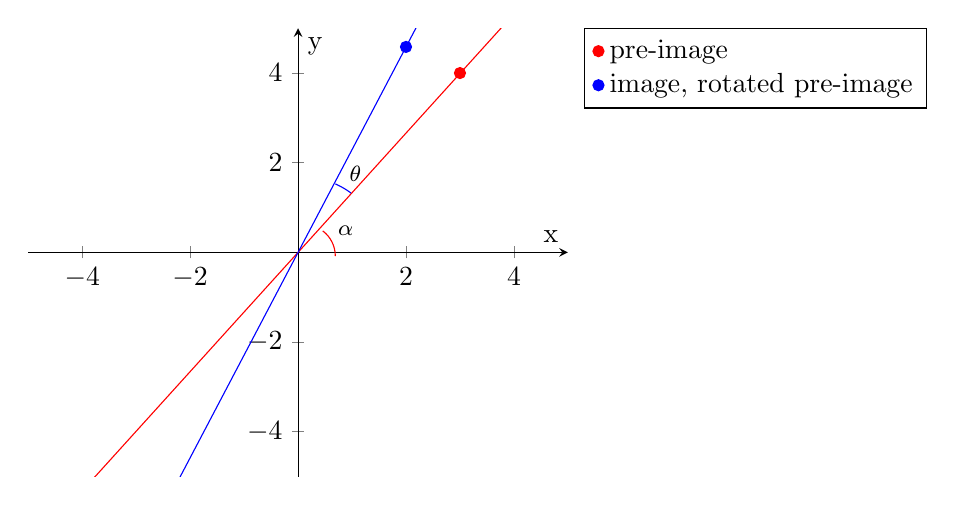
\begin{tikzpicture}
    \begin{axis}[
            axis lines = middle,
            xmin=-5, xmax=5,
            ymin=-5, ymax=5,
            xlabel = {x},
            ylabel = {y},
            legend pos=outer north east,
            legend cell align=left
        ]
        \addplot [only marks, color=red] table {
            3 4
        };
        \addlegendentry{pre-image}
        \addplot [only marks, color=blue] table {
            2 4.583
        };
        \addlegendentry{image, rotated pre-image}
        \addplot [color=red] {
            1.33 * x
        };
        \addplot [color=blue] {
            2.291 * x
        };
        \coordinate (origin) at (0,0);
    \end{axis}
    \begin{scope}[shift={(3.5, 2.8)}]
        \coordinate (O) at (0, 0);
        \coordinate (A) at (3, 4);
        \coordinate (B) at (2, 4.583);
        \draw[draw=blue] (O) ++(53.13:1) arc (53.13:66.42:1)
            node[midway,above right,inner sep=2pt,font={\footnotesize}]{$\theta$};
        \draw[draw=red] (O) ++(53.13:0.4) arc (53.13:0:0.4)
            node[midway,above right,inner sep=2pt,font={\footnotesize}]{$\alpha$};
    \end{scope}
\end{tikzpicture}
            \end{center}
        %\end{ln-fig} 

        Here, let us denote the pre-image $(x, y)$, and the rotated image $(x', y')$.
        The distance between $(x, y)$ and origin is same with the distance between $(x', y')$ with origin, which we will denote as:
        \[r = distance((x, y), (0, 0)) = distance((x', y'), (0, 0))\]
        Using high-school trigonometry, we can first make the following statements:
        \begin{align*}
            x = r \cos(\alpha) &, y = r \sin(\alpha) \\
            x' = r \cos(\alpha + \theta) &, y' = r \sin(\alpha + \theta)
        \end{align*}
        Later, using the angle summation formula, we may derive the relationship between $x$ and $x'$:
        \begin{align*}
            \cos(x + y) &= \cos(x)\cos(y) - \sin(x)\sin(y) \\
            x' &= r \cos(\alpha + \theta) \\
            &= r\cos(\alpha)\cos(\theta) - r\sin(\alpha)\sin(\theta) \\
            &= x\cos(\theta) - y\sin(\theta)
        \end{align*}
        Then, the relationship between $y$ and $y'$:
        \begin{align*}
            \sin(x + y) &= \sin(x)\cos(y) + \cos(x)\sin(y) \\
            y' &= r \sin(\alpha + \theta) \\
            &= r\sin(\alpha)\cos(\theta) + r\cos(\alpha)\sin(\theta) \\
            &= y\cos(\theta) + x\sin(\theta)
        \end{align*}
        So put in a system of equation, then a matrix-vector multiplication:
        \begin{align*}
            &\begin{cases}
                x' = x\cos(\theta) - y\sin(\theta) \\
                y' = y\cos(\theta) + x\sin(\theta)
            \end{cases} \\
            \begin{bmatrix} x' \\ y' \end{bmatrix} &=
            \begin{bmatrix}
                \cos(\theta) & -\sin(\theta) \\
                \sin(\theta) & \cos(\theta)
            \end{bmatrix}
            \begin{bmatrix} x \\ y \end{bmatrix} 
        \end{align*}
    }
    
    \item {
        Can you undo a rotation for any angle? Why or why not?
        
    }
    \meta {
        \begin{itemize}
            \item Mentors can feel free to \textbf{abstract away the math first} and use a graphical viewpoint to show that a rotation can be undoed by rotating the point back to its original position.
            \item The mathematical viewpoint of the solution exists to offer an \textbf{insight on the invertibility of rotation matrix and its proof}. If you are a student who reads our meta section, don't worry about the word invertibility until it appears in lecture.
            \item The solution \textbf{uses a function viewpoint to describe the linear transformation for rotation}. Feel free to use other views. The solution is using function for the sake of connecting with MATH 54 customs.
        \end{itemize}
        
    }
    \ans {
        Let us define the rotation matrix that rotates a point by angle $\theta$ counterclockwise as $r(\theta)$. \\
        Then, let us define the function $R(\vec{x}, \theta)$ to receive a vector $\vec{x}$ representing a coordinate and return the result of its rotation by angle $\theta$ counterclockwise. \\
        The result of a rotation is:
        \[
            R \bigg( \begin{bmatrix} x \\ y \end{bmatrix}, \theta \bigg) =
            \begin{bmatrix} x' \\ y' \end{bmatrix} =
            \begin{bmatrix}
                \cos(\theta) & -\sin(\theta) \\
                \sin(\theta) & \cos(\theta)
            \end{bmatrix}
            \begin{bmatrix} x \\ y \end{bmatrix}
        \]
        If we \textbf{rotate the same point by the same angle back, which means rotating a point by angle $\theta$ clockwise}, then the point ought to return to its original coordinates. Rotating by an angle $\theta$ clockwise is equivalent to rotating by an angle $-\theta$ counterclockwise. Therefore, such a rotation would be expressed as $R(\vec{x}, -\theta)$. \\
        Now, let us \textbf{mathematically show that rotating a point by angle $\theta$ counterclockwise, then rotating by an angle $-\theta$ counterclockwise will undo the prior rotation}:
        \begin{align*}
            R \bigg( \begin{bmatrix} x \\ y \end{bmatrix}, \theta \bigg)
            &= 
            \begin{bmatrix} x' \\ y' \end{bmatrix}
            =
            \begin{bmatrix}
                \cos(\theta) & -\sin(\theta) \\
                \sin(\theta) & \cos(\theta)
            \end{bmatrix}
            \begin{bmatrix} x \\ y \end{bmatrix} \\
            R \bigg( R \bigg( \begin{bmatrix} x \\ y \end{bmatrix}, \theta \bigg), -\theta \bigg)
            &=
            \begin{bmatrix}
                \cos(-\theta) & -\sin(-\theta) \\
                \sin(-\theta) & \cos(-\theta)
            \end{bmatrix}
            \begin{bmatrix}
                \cos(\theta) & -\sin(\theta) \\
                \sin(\theta) & \cos(\theta)
            \end{bmatrix}
            \begin{bmatrix} x \\ y \end{bmatrix} \\
            &=
            \begin{bmatrix}
                \cos(\theta) & \sin(\theta) \\
                -\sin(\theta) & \cos(\theta)
            \end{bmatrix}
            \begin{bmatrix}
                \cos(\theta) & -\sin(\theta) \\
                \sin(\theta) & \cos(\theta)
            \end{bmatrix}
            \begin{bmatrix} x \\ y \end{bmatrix} \\
            &=
            \begin{bmatrix}
                \cos^2(\theta) + \sin^2(\theta) & 
                \cos(\theta)\sin(\theta) - \cos(\theta)\sin(\theta) \\
                \cos(\theta)\sin(\theta) - \cos(\theta)\sin(\theta) &
                \sin^2(\theta) + \cos^2(\theta)
            \end{bmatrix}
            \begin{bmatrix} x \\ y \end{bmatrix} \\
            &=
            \begin{bmatrix} x \\ y \end{bmatrix}
        \end{align*}
    
    }
    
    \item {
        Describe the following transformations, and explain whether they are undoable.
        \begin{tasks}(2)
            \task[(i)] $
                    \begin{bmatrix} x' \\ y' \end{bmatrix} = 
                    \begin{bmatrix}
                       1 & 0 \\
                       0 & -1
                    \end{bmatrix}
                    \begin{bmatrix} x \\ y \end{bmatrix}
            $
            \task[(ii)] $
                    \begin{bmatrix} x' \\ y' \end{bmatrix} = 
                    \begin{bmatrix}
                       -1 & 0 \\
                       0 & 1
                    \end{bmatrix}
                    \begin{bmatrix} x \\ y \end{bmatrix}
            $ \\
            \task[(iii)] $
                \begin{bmatrix} x' \\ y' \\ z' \end{bmatrix} = 
                \begin{bmatrix}
                    2 & 0 & 0 \\
                    0 & 3 & 0 \\
                    0 & 0 & 0 \\
                \end{bmatrix}
                \begin{bmatrix} x \\ y \\ z \end{bmatrix}
            $
            \task[(iv)] $
                \begin{bmatrix} x' \\ y' \end{bmatrix} = 
                \begin{bmatrix}
                   2 & 0 \\
                   0 & 3
                \end{bmatrix}
                \begin{bmatrix}
                    cos(\theta) & -sin(\theta) \\
                    sin(\theta) & cos(\theta)
                \end{bmatrix}
                \begin{bmatrix} x \\ y \end{bmatrix}
            $
        \end{tasks}
        
        
    }
    \meta {
        \begin{itemize}
            \item The question comes down to:
            \subitem - \textbf{Describe} the transformation
            \subitem - \textbf{Show examples} of transformation results.
            \subitem - Is it possible to \textbf{find the point's original location based on its transformed location}?
            \item \textbf{Subpart (iii) is a hint at "Loss of Dimensionality"}, which will be introduced upon learning the term "nullspace" (or "kernel").
            \item \textbf{Subpart (iv) is a hint at non-commutativeness}. See if the transformation is same if we switched the order of matrices.
            \item These questions' \textbf{presentation highly depends on the pedagogy of mentor}.
        \end{itemize}
        
    }
    \ans {
        Alright, so. \textbf{Let's get rotated.}
        \begin{enumerate}
            \item {
                For every pre-image $(x, y)$, the image is $(x, -y)$. \\
                This means we have reflected the point across the x-axis:
                \begin{ln-fig}{The Rotation of a Point across x-Axis}{}
                    \begin{center}
                        \input{../../topics/matrix_multiplication/q_rotate_reflect_matrix_figs/point_reflect_x.tex}
                    \end{center}
                \end{ln-fig}
                To undo this reflection, we would reflect the image across the x-axis again:
                \[
                    \begin{bmatrix}
                       1 & 0 \\
                       0 & -1
                    \end{bmatrix}
                    \begin{bmatrix}
                       1 & 0 \\
                       0 & -1
                    \end{bmatrix}
                    \begin{bmatrix} x \\ y \end{bmatrix} =
                    \begin{bmatrix}
                       1 & 0 \\
                       0 & 1
                    \end{bmatrix}
                    \begin{bmatrix} x \\ y \end{bmatrix} =
                    \begin{bmatrix} x \\ y \end{bmatrix}
                \]
            }
            \item {
                For every pre-image $(x, y)$, the image is $(-x, y)$. \\
                This means we have reflected the point across the y-axis:
                \begin{ln-fig}{The Rotation of a Point across y-Axis}{}
                    \begin{center}
                        % Author: Dun-Ming Huang
% Email: dunmingbrandonhuang@berkeley.edu
% CSM16A Fall 2022

\begin{tikzpicture}
    \begin{axis}[
            axis lines = middle,
            xmin=-5, xmax=5,
            ymin=-5, ymax=5,
            xlabel = {x},
            ylabel = {y},
            legend pos=outer north east,
            legend cell align=left
        ]
        \addplot [only marks, color=red] table {
            2 2
            3 4
            -1 3
            -5 -3
        };
        \addlegendentry{pre-image}
        \addplot [only marks, color=blue] table {
            -2 2
            -3 4
            1 3
            5 -3
        };
        \addlegendentry{image, reflected pre-image}
    \end{axis}
\end{tikzpicture}
                    \end{center}
                \end{ln-fig}
                To undo this reflection, we would reflect the image across the y-axis again:
                \[
                    \begin{bmatrix}
                       -1 & 0 \\
                       0 & 1
                    \end{bmatrix}
                    \begin{bmatrix}
                       -1 & 0 \\
                       0 & 1
                    \end{bmatrix}
                    \begin{bmatrix} x \\ y \end{bmatrix} =
                    \begin{bmatrix}
                       -1 & 0 \\
                       0 & 1
                    \end{bmatrix}
                    \begin{bmatrix} x \\ y \end{bmatrix} =
                    \begin{bmatrix} x \\ y \end{bmatrix}
                \]
            }
            \item {
                For every pre-image $(x, y, z)$, the image is $(2x, 3y, 0)$. \\
                Let us demonstrate with some examples below:
                \begin{ln-fig}[sidebyside]{The Results of Transformation c-iii}{}
                    \begin{center}
                        % Author: Dun-Ming Huang
% Email: dunmingbrandonhuang@berkeley.edu
% CSM16A Fall 2022
 %Code references works on Anna Chou's work in EECS 16A CSM Question Bank
 
 \begin{tikzpicture}[x=1cm, y=1cm, z=-0.6cm]
    % Axes
    \draw [->] (0,0,0) -- (0,0,4) node [left] {$x$};
    \draw [->] (0,0,0) -- (3.5,0,0) node [above] {$y$};
    \draw [->] (0,-2,0) -- (0,0,0) -- (0,2,0) node [above] {$z$};
    
    % Ticks
        \foreach \i in {1,2,3}
    {
    \draw (\i,-0.1,0) -- ++ (0,0.2,0);
    \draw (-0.1,0,\i) -- ++ (0.2,0,0);
    }
        \foreach \i in {1, 2}
    {
        \draw (-0.1,\i,0) -- ++ (0.2,0,0);
        \draw (-0.1,-\i,0) -- ++ (0.2,0,0);
    }
    % Dashed lines
    \draw [loosely dashed, draw=red]
        (0,0,1) -- (1,0,1) -- (1,0,0)
        (0,1,0) -- (0,1,1) -- (0,0,1)
        (1,0,0) -- (1,1,0) -- (0,1,0)
        (1,1,0) -- (1,1,1) -- (0,1,1)
        (1,1,1) -- (1,0,1)
        ;
    \draw [loosely dashed, draw=blue]
        (3,0,0) -- (3,0,2) -- (0,0,2)
        ;
    % Labels
     \node [below right, label={[font=\small,text=red]30:pre-image}] at (1.5,1,1) {};
     \node [below right, label={[font=\small,text=blue]30:image}] at (1.5,-1, 1.2) {};
\end{tikzpicture}
                    \end{center}
                    \tcblower
                    \begin{center}
                        % Author: Dun-Ming Huang
% Email: dunmingbrandonhuang@berkeley.edu
% CSM16A Fall 2022
%Code references works on https://tex.stackexchange.com/questions/348609/draw-a-3d-sphere-with-radius-with-tikz

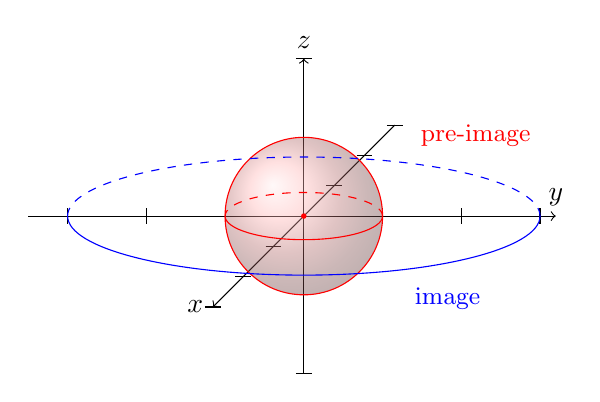
\begin{tikzpicture}
    % Axes
    \draw [->] (0,0,-3) -- (0,0,3) node [left] {$x$};
    \draw [->] (-3.5,0,0) -- (3.2,0,0) node [above] {$y$};
    \draw [->] (0,-2,0) -- (0,0,0) -- (0,2,0) node [above] {$z$};
    
    % Ticks
        \foreach \i in {-3, -2, -1, 1,2,3}
    {
    \draw (\i,-0.1,0) -- ++ (0,0.2,0);
    \draw (-0.1,0,\i) -- ++ (0.2,0,0);
    }
        \foreach \i in {1, 2}
    {
        \draw (-0.1,\i,0) -- ++ (0.2,0,0);
        \draw (-0.1,-\i,0) -- ++ (0.2,0,0);
    }
    
    % Sphere
    \shade[ball color = red!40, opacity = 0.4] (0,0) circle (1cm);
    \draw[draw=red] (0,0) circle (1cm);
    \draw[draw=red] (-1,0) arc (180:360:1 and 0.3);
    \draw[dashed, draw=red] (1,0) arc (0:180:1 and 0.3);
    \fill[fill=red] (0,0) circle (1pt);
    \draw[draw=blue] (-3,0) arc (180:360:3 and 0.75);
    \draw[dashed, draw=blue] (3,0) arc (0:180:3 and 0.75);
    
    % labels
    \node [below right, label={[font=\small,text=red]30:pre-image}] at (1.5,1.2,1) {};
    \node [below right, label={[font=\small,text=blue]30:image}] at (1.5,-0.8, 1.2) {};
    
\end{tikzpicture}
                    \end{center}
                \end{ln-fig}
                In the above solids (which are sets of three-dimensional coordinates), while every point's x-coordinate is doubled and y-coordinate is tripled (as stated in the first sentence of the solution), the z-coordinate is gone. \\
                In other words, our \textbf{solids have both lost one dimension. There is a reduction of dimensionality.} \\
                We also have \textbf{no information about how to restore the image back to the pre-image}, since there is no clue regarding the original $z$-coordinate of each point if we are only provided the pre-image. Not knowing how to provide each point the correct height, we cannot undo the above transformation.
            }
            \item{
                Let us observe this transformation matrix-by-matrix, because graphing out the points with transformations of multiple matrices is tedious to do by hand during assignments and exams. \\
                The rightmost transformation matrix that is first multiplied by the coordinate $(x, y)$ is a rotation matrix. The second multiplied matrix is a dilation matrix that dilates the original point and converts a coordinate $(a, b)$ into $(2a, 3b)$. \\
                In other words, this transformation is a chain of operations, where we first rotate a point, then dilate it. \\
                To undo it, we can dilate it by another dilation matrix that undoes the original dilation:
                \[
                    \begin{bmatrix}
                       \frac{1}{2} & 0 \\
                       0 & \frac{1}{3}
                    \end{bmatrix}
                \]
                and then rotate it by the same angle $\theta$ but clockwise (as we have described in part (b)).
            }
        \end{enumerate}
        The property of being an undo-able transformation has a name. You will see it soon in lectures!
        
    }
    
    \item{
        Take a break.
        
    }
    
    \meta{
        \begin{itemize}
            \item Starting from here, we are \textbf{entering the non-review section}.
            \item The following problems \textbf{simulate a medium to high difficulty exam/assignment problem}. While valuing independent work due to the nature of exams, \textbf{mentors are encouraged to guide students} through some of the more difficult problems. 
            \item For mentors, to \textbf{check your work on whether the rotation seems correct, please utilize the dot product angle formula}. If you are a student who is reading this meta point, don't worry about what a "dot product angle formula" is. You either fortunately learned in from pre-calculus or will have to wait for its appearance in November.
        \end{itemize}
        
    }
    
    \item {
        Rotate the line $y = 3x$ around the origin ${45}^{\circ}$ clockwise, what is its linear equation? \\
        \textit{(Hint: to rotate a line is to rotate every single point on it, and \textbf{find the relationship between} $x$ and $y$, and then $x'$ and $y'$.)}
        
    }
    \meta {
        The \textbf{approach to this problem comes down to}:
        \begin{itemize}
            \item Each point on the line $y = 3x$ can be described as $(x, y)$
            \item Rotate an arbitrary point $(x, y)$ will provide us a coordinate $(x', y')$, where $x'$, $y'$ are new coordinates in terms of trigonometric functions and $x$, $y$.
            \item We know that $y = 3x$, and both $x$ and $y$ can also be expressed in terms of $x'$ and $y'$.
            \item Solve for an equation in terms of $x'$ and $y'$ applying the above.
        \end{itemize}
        
    }
    \ans {
        Let us express an arbitrary point on the line $y=3x$ as $\begin{bmatrix} x & y \end{bmatrix}^T$. \\
        Then, to rotate this point on the line by by the origin by $45^{\circ}$ counterclockwise, we will apply the transformation matrix on it:
        \begin{align*}
            \begin{bmatrix} x' \\ y' \end{bmatrix} 
            &=
            \begin{bmatrix}
                cos({45}^{\circ}) & -sin({45}^{\circ}) \\
                sin({45}^{\circ}) & cos({45}^{\circ})
            \end{bmatrix}
            \begin{bmatrix} x \\ y \end{bmatrix} \\
            &=
            \begin{bmatrix}
                \frac{1}{\sqrt{2}} & -\frac{1}{\sqrt{2}} \\
                \frac{1}{\sqrt{2}} & \frac{1}{\sqrt{2}}
            \end{bmatrix}
            \begin{bmatrix} x \\ y \end{bmatrix}
        \end{align*}
        Here, we can comprehend the coordinates $\begin{bmatrix} x & y \end{bmatrix}^T$ as the coordinates of points the new line should contain.\\
        In other words, they are the results of rotations:
        \begin{ln-fig}{A Graphical Representation of Rotating Lines}{}
            \begin{center}
                % Author: Dun-Ming Huang
% Email: dunmingbrandonhuang@berkeley.edu
% CSM16A Fall 2022

\begin{center}
    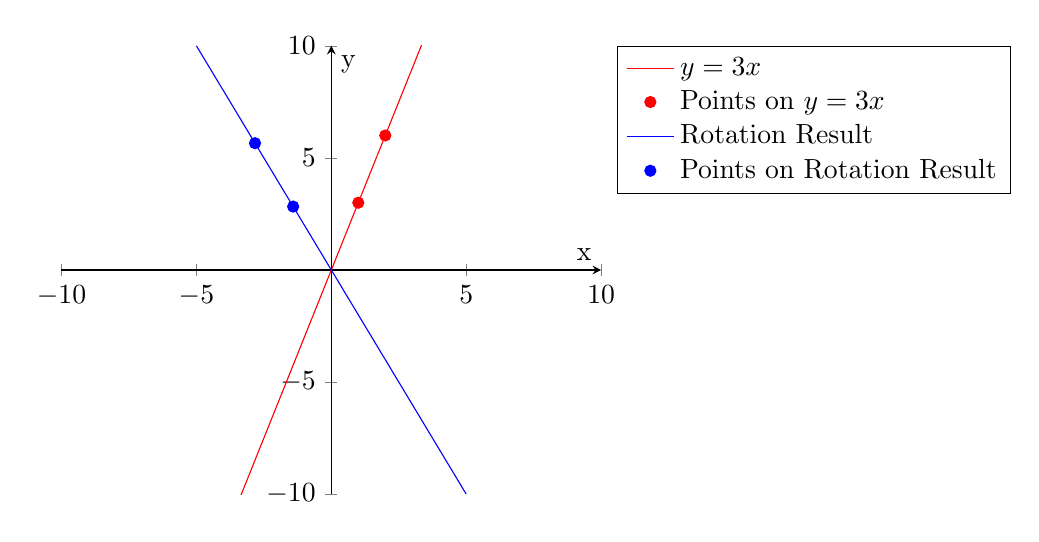
\begin{tikzpicture}
        \begin{axis}[
            axis lines = middle,
            xmin=-10, xmax=10,
            ymin=-10, ymax=10,
            xlabel = {x},
            ylabel = {y},
            legend pos=outer north east,
            legend cell align=left
        ]
            \addplot [color=red] {
               3*x
            };
            \addlegendentry{$y = 3x$}
            \addplot [only marks, color=red] table {
               1 3
               2 6
            };
            \addlegendentry{Points on $y = 3x$}
            \addplot [color=blue] {
                -2*x
            };
            \addlegendentry{Rotation Result}
            \addplot [only marks, color=blue] table {
               -1.414 2.828
               -2.828 5.656
            };
            \addlegendentry{Points on Rotation Result}
        \end{axis}
    \end{tikzpicture}
\end{center}
            \end{center}
        \end{ln-fig}
        Applying the undoing of the rotation matrix (which is a rotation clockwise by ${45}^{\circ}$) on both sides of above equation:
        \begin{align*}
            \begin{bmatrix} x' \\ y' \end{bmatrix} 
            &=
            \begin{bmatrix}
                cos(-{45}^{\circ}) & -sin(-{45}^{\circ}) \\
                sin(-{45}^{\circ}) & cos(-{45}^{\circ})
            \end{bmatrix}
            \begin{bmatrix} x \\ y \end{bmatrix} \\
            &=
            \begin{bmatrix} x \\ y \end{bmatrix} =
            \begin{bmatrix}
                \frac{1}{\sqrt{2}} & \frac{1}{\sqrt{2}} \\
                -\frac{1}{\sqrt{2}} & \frac{1}{\sqrt{2}}
            \end{bmatrix}
            \begin{bmatrix} x' \\ y' \end{bmatrix}
        \end{align*}
        Therefore, the relationship between the points on original line $(x, y)$ and the points on the rotated line $(x', y')$ can be expressed:
        \[
            \begin{cases}
                x = \frac{1}{\sqrt{2}}x' + \frac{1}{\sqrt{2}}y' \\
                y = -\frac{1}{\sqrt{2}}x' + \frac{1}{\sqrt{2}}y'
            \end{cases}
        \]
        And since we know that the points on the original line must satisfy the condition $y=3x$:
        \begin{align*}
            y
            = -\frac{1}{\sqrt{2}}x' + \frac{1}{\sqrt{2}}y'
            &= 3(\frac{1}{\sqrt{2}}x' + \frac{1}{\sqrt{2}}y') = 3x \\
            \sqrt{2}(-\frac{1}{\sqrt{2}}x' + \frac{1}{\sqrt{2}}y')
            &= 3(\frac{1}{\sqrt{2}}x' + \frac{1}{\sqrt{2}}y') \\
            -x' + y' &= 3x' + 3y' \\
            y' &= -2x'
        \end{align*}
        Therefore, since all points of the rotated lines satisfy the conditions $y' = -2x'$, the rotated line's linear equation would be:
        \[y = -2x\]
        
    }
    
    \item {
        Rotate the line $y = 3x$ \textbf{around the point $(1, 1)$}, ${30}^{\circ}$ clockwise. \\
        (Discuss with your classmate(s)!)
        
    }
    \meta {
        \begin{itemize}
            \item We are \textbf{not rotating by the origin this time}. We are \textbf{\textit{not rotating by the origin this time}}.
            \item The solution outlines 2 approaches to think of. But the \textbf{main idea is always: make a temporary translation, perform rotation, undo the temporary translation}.
            \item This process can also be \textbf{described as an "algorithm"}.
        \end{itemize}
        
    }
    \ans {
        While we know how to rotate a graph by the origin, we don't know how to rotate a graph using other points as the center of rotation, and also don't want to take time into deriving it. To overcome this, we must find ways such that we can make treat the current center of rotation as some form of origin. \\
        So, there stems two approaches: \\
        
        \textbf{Approach 1: Translate the Coordinate Axes}
        \begin{ln-fig}{Translating the Coordinate Axes and Pre-Image}{}
            \begin{center}
                % Author: Dun-Ming Huang
% Email: dunmingbrandonhuang@berkeley.edu
% CSM16A Fall 2022

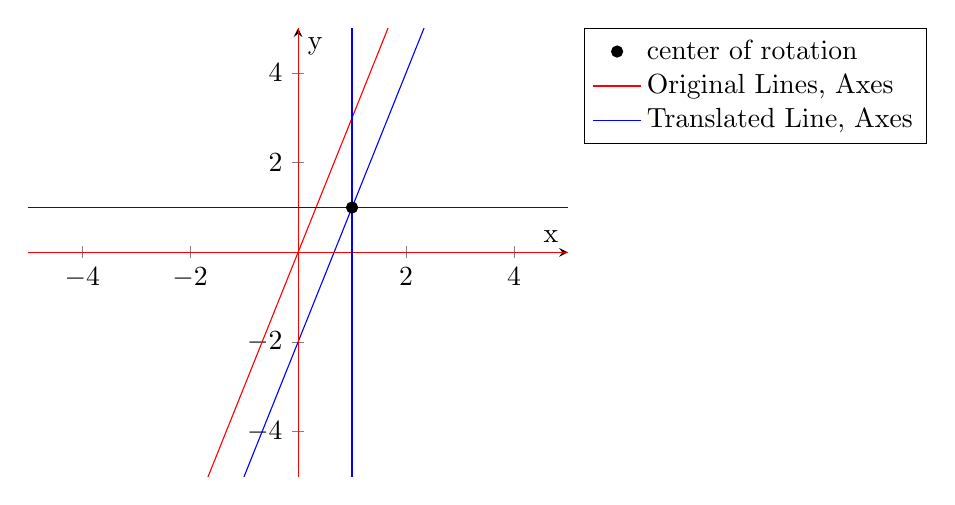
\begin{tikzpicture}
    \begin{axis}[
        axis lines = middle,
        xmin=-5, xmax=5,
        ymin=-5, ymax=5,
        xlabel = {x},
        ylabel = {y},
        legend pos=outer north east,
        legend cell align=left
    ]
        \addplot [only marks, color=black] table {
            1 1
        };
        \addlegendentry{center of rotation}
        \addplot [color=red] {
           3*x
        };
        \addlegendentry{Original Lines, Axes}
        \addplot [color=blue] {
           3*x - 2
        };
        \addlegendentry{Translated Line, Axes}
        \addplot [color=red] {
           0
        };
        \addplot [color=red] coordinates {
            (0, -5) (0, 5)
        };
        \addplot [color=blue] {
           1
        };
        \addplot [color=blue] coordinates {
            (1, -5) (1, 5)
        };
    \end{axis}
\end{tikzpicture}
    
            \end{center}
        \end{ln-fig}
        We translated the coordinate axes such that the new origin of this system is the current center of rotation: $(1, 1)$. Because of that, every point's x and y coordinate each decreases by 1 in the new coordinate system:
        \[
            \begin{bmatrix} x' \\ y' \end{bmatrix} = 
            \begin{bmatrix} x \\ y \end{bmatrix} - \begin{bmatrix} 1 \\ 1 \end{bmatrix}
        \]
        Now that \textbf{the center of rotation is the origin of the new coordinate system}, our next move follows:
        \begin{ln-fig}{Rotate the Line by the Center of Rotation}{}
            \begin{center}
                % Author: Dun-Ming Huang
% Email: dunmingbrandonhuang@berkeley.edu
% CSM16A Fall 2022

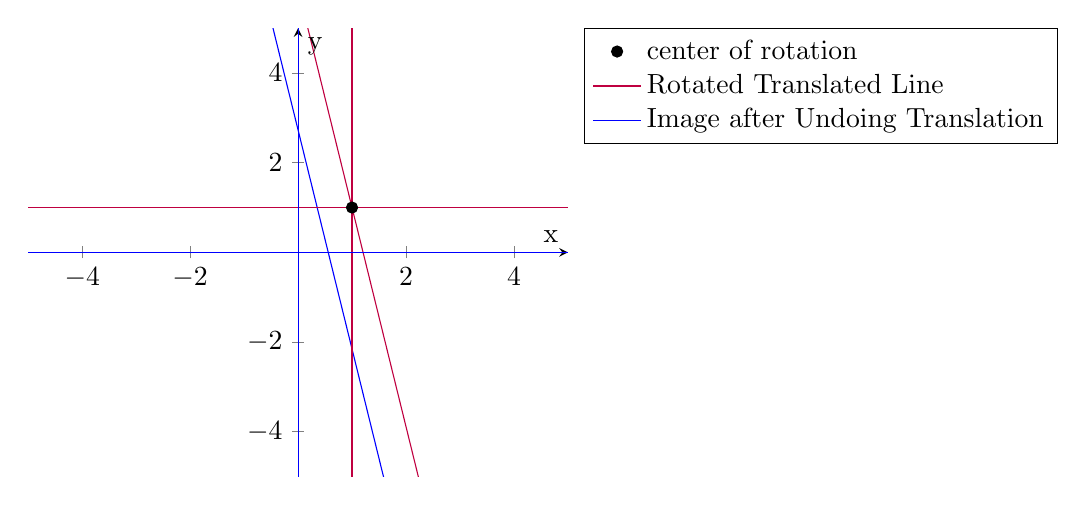
\begin{tikzpicture}
    \begin{axis}[
        axis lines = middle,
        xmin=-5, xmax=5,
        ymin=-5, ymax=5,
        xlabel = {x},
        ylabel = {y},
        legend pos=outer north east,
        legend cell align=left
    ]
        \addplot [only marks, color=black] table {
            1 1
        };
        \addlegendentry{center of rotation}
        \addplot [color=purple] {
           (6.196*x - 7.464) / -1.268
        };
        \addlegendentry{Rotated Translated Line}
        \addplot [color=blue] {
            (6.196*x - 3.464) / -1.268
        };
        \addlegendentry{Image after Undoing Translation}
        \addplot [color=purple] {
           1
        };
        \addplot [color=purple] coordinates {
            (1, -5) (1, 5)
        };
        \addplot [color=blue] {
           0
        };
        \addplot [color=blue] coordinates {
            (0, -5) (0, 5)
        };
        
    \end{axis}
\end{tikzpicture}
            \end{center}
        \end{ln-fig}
        Then we rotated the line by the center of rotation, which we can directly apply the rotation matrix onto because now the origin is the center of rotation. Afterwards, we revert the translation of axes done in first step by moving the axes left and down 1 unit, which consequently adds each points' x and y coordinates by 1.
        
        \textbf{Approach 2: translate the entire graph}
        \begin{ln-fig}{Translate the Graph Down by $(1, 1)$}{}
            \begin{center}
                % Author: Dun-Ming Huang
% Email: dunmingbrandonhuang@berkeley.edu
% CSM16A Fall 2022

\begin{tikzpicture}
    \begin{axis}[
        axis lines = middle,
        xmin=-5, xmax=5,
        ymin=-5, ymax=5,
        xlabel = {x},
        ylabel = {y},
        legend pos=outer north east,
        legend cell align=left
    ]
        \addplot [color=red] {
           3*x
        };
        \addlegendentry{Pre-Image}
        \addplot [color=blue] {
           3*x + 2
        };
        \addlegendentry{Translated Pre-Image}
        \addplot [only marks, color=red] table {
            1 1
        };
        \addplot [only marks, color=blue] table {
            0 0
        };
    \end{axis}
\end{tikzpicture}

            \end{center}
        \end{ln-fig}
        This time, we translated the entire graph with the center of rotation instead of moving the axes, so our center of rotation is at the origin now. This causes every point to be move lower and left by 1 unit:
        \[
            \begin{bmatrix} x' \\ y' \end{bmatrix} = 
            \begin{bmatrix} x \\ y \end{bmatrix} - \begin{bmatrix} 1 \\ 1 \end{bmatrix}
        \]
        \begin{ln-fig}{Rotate the Line by Center of Rotation}{}
            \begin{center}
                % Author: Dun-Ming Huang
% Email: dunmingbrandonhuang@berkeley.edu
% CSM16A Fall 2022

\begin{tikzpicture}
    \begin{axis}[
        axis lines = middle,
        xmin=-5, xmax=5,
        ymin=-5, ymax=5,
        xlabel = {x},
        ylabel = {y},
        legend pos=outer north east,
        legend cell align=left
    ]
        \addplot [color=violet] {
           (6.196*x + 4) / -1.268
        };
        \addlegendentry{Rotated Translated Pre-Image}
        \addplot [color=pink!30!black!50!] {
           (6.196*x - 3.464) / -1.268
        };
        \addlegendentry{Translation Undo'ed, Final Image}
        \addplot [only marks, color=violet] table {
            0 0
        };
        \addplot [only marks, color=pink!30!black!50!] table {
            1 1
        };
    \end{axis}
\end{tikzpicture}

            \end{center}
        \end{ln-fig}
        As done before, we \textbf{then rotate the line by the origin} (which is now the center of origin due to the translation), and \textbf{then revert the first translation} so our graph and center of rotation is back to where it should be.
        
        Either way, the step of transformations would follow the same mathematical form:
        \begin{ln-quest}{The Steps of Rotating a Point around $(1, 1)$ by ${30}^{\circ}$}{}
            \textbf{Step 1}: Translation
            \[
                \begin{bmatrix} x' \\ y' \end{bmatrix} = 
                \begin{bmatrix} x \\ y \end{bmatrix} - \begin{bmatrix} 1 \\ 1 \end{bmatrix}
            \]
            \textbf{Step 2}: Rotation
            \[
                \begin{bmatrix} x'' \\ y'' \end{bmatrix} = 
                R(30^{\circ})
                \begin{bmatrix} x' \\ y' \end{bmatrix}
            \]
            \textbf{Step 3}: Undo-translation
            \[
                \begin{bmatrix} x''' \\ y''' \end{bmatrix} = 
                R(30^{\circ})
                \begin{bmatrix} x'' \\ y'' \end{bmatrix} + \begin{bmatrix} 1 \\ 1 \end{bmatrix}
            \]
            The final solution is the coordinate $\begin{bmatrix} x''' \\ y''' \end{bmatrix}$
        \end{ln-quest}
        
        
        So, expressing $(x', y')$ as the final result of transformation from $(x, y)$, an arbitrary original point on the line:
        \[
            \begin{bmatrix} x' \\ y' \end{bmatrix}
            = R(30^{\circ})
            \begin{bmatrix} x - 1 \\ y - 1 \end{bmatrix} + 
            \begin{bmatrix} 1 \\ 1 \end{bmatrix}
        \]
        Which means, while $y = 3x$,
        \[
            \begin{bmatrix} x \\ y \end{bmatrix}
            = R^{-1}(30^{\circ})
            \begin{bmatrix} x' - 1 \\ y' - 1 \end{bmatrix} + 
            \begin{bmatrix} 1 \\ 1 \end{bmatrix}
        \]
        So now, deriving for the linear equation:
        \[
            (3\sqrt{3} + 1)x - 2\sqrt{3} = (\sqrt{3} - 3)y
        \]
        
    }
    
    \item {
        Discuss with your classroom, and come up with an algorithm for reflecting a point across a line $y = 3x$. \\
        Is this operation undoable? Why or why not?
        
    }
    \meta {
        \begin{itemize}
            \item This \textbf{question is long}.
            \item But, its \textbf{spirit is actually the same with part (e)}. We just \textbf{replaced the temporary translation with a temporary rotation}.
            \item So the suggestions for going through this problem is essentially identical to that for the previous part.
        \end{itemize}
        
    }
    \ans {
        Before we actually solve this problem, let us think of a problem-solving process for this function, step-by-step: 
    	\begin{enumerate}
    	    \item {
        	    \textit{How can I describe reflecting a point $(x,y)$ across the x-axis with a matrix $R$, such that, for the new coordinates of the point $(x',y')$:}
        	    \[
        	        \begin{bmatrix} x' \\ y' \end{bmatrix} =
        	        R \begin{bmatrix} x \\ y \end{bmatrix}
        	    \]
        	}
        	\begin{ln-fig}{Reflecting a Point Across x-Axis}{}
        	    \begin{center}
        	        % Author: Dun-Ming Huang
% Email: dunmingbrandonhuang@berkeley.edu
% CSM16A Fall 2022

\begin{center}
    \begin{tikzpicture}
        \begin{axis}[
            axis lines = middle,
            xmin=-5, xmax=5,
            ymin=-5, ymax=5,
            xlabel = {x},
            ylabel = {y},
            legend pos=outer north east,
            legend cell align=left
        ]
            \addplot [only marks, color=red] table {
                1 1
                2 2
                3 4
            };
            \addlegendentry{pre-image}
            \addplot [only marks, color=blue] table {
                1 -1
                2 -2
                3 -4
            };
            \addlegendentry{image}
        \end{axis}
    \end{tikzpicture}
\end{center}
        	    \end{center}
        	\end{ln-fig}
            By reflecting a point across the x-axis, while its x coordinate will not be changed, its y coordinate will become the original's opposite value.
            
            
            In terms of matrix transformation, with $(x, y)$ being the original coordinate and $(x', y')$ being the transformed (reflected) coordinate, it can be expressed that:
            \[
                \begin{bmatrix} x' \\ y' \end{bmatrix} = 
                \begin{bmatrix}
                    1 & 0 \\
                    0 & -1
                \end{bmatrix}
                \begin{bmatrix} x \\ y \end{bmatrix}
            \]
                
    	    \item {
    	        \textit{What can I do to reduce this situation from reflecting a point across the line $y = mx$ to reflecting a point across the x-axis? How do I cancel that transformation?}
    	        \begin{ln-fig}{Reflecting a Point across $y = mx$}{}
                	\begin{center}
                	    \input{../../topics/matrix_multiplication/q_rotate_reflect_matrix_figs/point_across_line}
                	\end{center}
                \end{ln-fig}
    	    }
            I can rotate the entire figure by angle $\phi$ clockwise, such that this temporary rotation yields the result:
            \begin{ln-fig}{Reflecting a Point across $y = mx$, with Image}{}
                	\begin{center}
                	    % Author: Dun-Ming Huang
% Email: dunmingbrandonhuang@berkeley.edu
% CSM16A Fall 2022

\begin{center}
    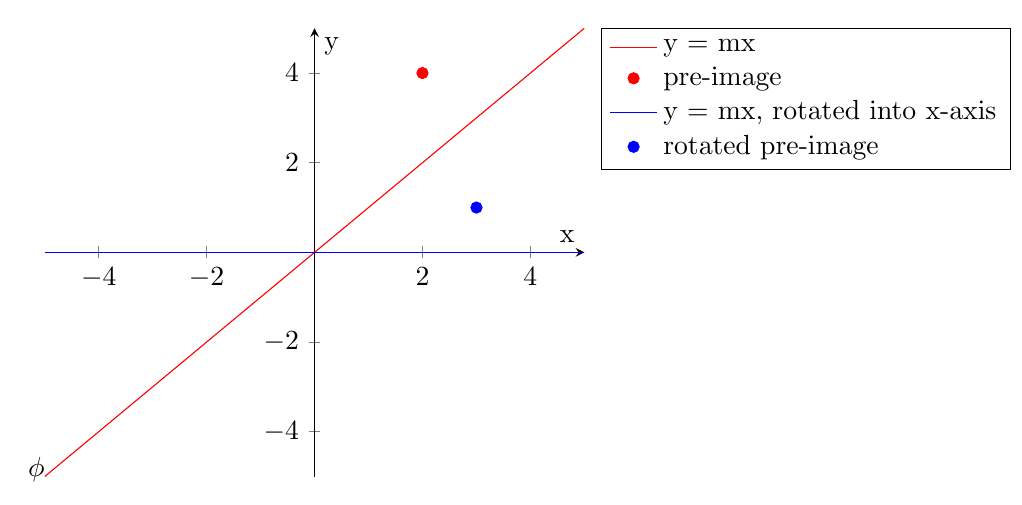
\begin{tikzpicture}
        \tkzDefPoint(3.5,2.8){O}
        \tkzDefPoint(6.5,5.8){A}
        \tkzDefPoint(6.5,2.8){B}
        \tkzMarkAngle[line width = 1.5pt, arrows = <-](B,O,A)
        \tkzLabelAngle[pos=1.5](B,O,A){$\phi$}
        \begin{axis}[
            axis lines = middle,
            xmin=-5, xmax=5,
            ymin=-5, ymax=5,
            xlabel = {x},
            ylabel = {y},
            legend pos=outer north east,
            legend cell align=left
        ]
            \addplot [color=red] {
               x
            };
            \addlegendentry{y = mx}
            \addplot [only marks, color=red] table {
                2 4
            };
            \addlegendentry{pre-image}
            \addplot [color=blue] {
               0
            };
            \addlegendentry{y = mx, rotated into x-axis}
            \addplot [only marks, color=blue] table {
                3 1
            };
            \addlegendentry{rotated pre-image}
        \end{axis}
    \end{tikzpicture}
\end{center}
                	\end{center}
                \end{ln-fig}
            Per description form Meta that might be invisible to students who receive this solution, "By doing so (the rotation of entire figure), it's equivalent that we have entered a new rotated version of coordinate plane. \\
            By reverting the rotation, we exit the new version of coordinate plane, into the original xy-plane system we are using." \\
            
            Why do we go through this part? \\
            The only information we currently have about how to reflect a point across a line is how the coordinates change when we reflect across the coordinate axes. We have not learned/derived anything regarding reflection across a diagonal line. \\
            
            So, what we may do is first reduce this situation into reflecting across a coordinate axis, and after we have done some intermediate transformations to reflect this point across the rotated version of $y = mx$, revert the original rotation we've done to the entire graph. \\
            
            The entire procedure of transformation then looks something to the lines of:
            \begin{ln-quest}{A Rough Draft for Point Reflection Algorithm}{}
                \begin{enumerate}[wide = 0pt]
                	\item [Step 1: ] Rotate the entire graph by angle $\phi$ clockwise
                	\item [Step 2, onwards: ] Some intermediate transformation occurs.
                	\item [Step Final: ] Revert the original rotation via rotating the entire graph by angle $\phi$ counterclockwise.
                \end{enumerate}
            \end{ln-quest}
      
    	    \item {
            	\textit{Combining the above knowledge, try describing a sequence of transformations we can apply onto the original point $(x_0,y_0)$, so we have reflected this point across the line $y = mx$.}
    	    }
    	    
    	    Continuing off part ii, after I commit the temporary rotation of the entire figure on coordinate plane, I reflect the point across the x-axis, and then revert the rotation such that we rotate the point by angle $\phi$ by the origin.
    	    
    	    \begin{ln-fig}{Full Graph-Based Summary of Point Reflection Algorithm}{}
    	        \begin{center}
                    \input{../../topics/matrix_multiplication/q_rotate_reflect_matrix_figs/point_across_line_algo}
                \end{center}
            \end{ln-fig}
            
        	In the above parts, you have described a step-by-step approach to resolve a problem. This step-by-step approach to resolve problems is known as an “algorithm”, and computers use algorithms because while computers are good at executing simple commands, they cannot directly perform complicated actions. \\
        	
        	The computer thinks in the pattern of executing one short command after another, thus, to reflect an image in a computer software, we would need to offer it an algorithm, so it has a sequence of instructions to work with.
        	
            \item {
                \textit{Finally, describe and summarize the algorithm for reflecting a point in terms of one transformation matrix.}
        	}
        	
        	We would need this along the way:
    	    \[
    	        \begin{cases}
    	            cos(2\theta) = cos^2(\theta) - sin^2(\theta) \\
    	            sin(2\theta) = 2sin(\theta)cos(\theta)
    	        \end{cases}
    	    \]
            For all points in pre-image:
            \begin{ln-quest}{Mathematical Summary of Point Reflection Algorithm}{}
                \begin{enumerate}[wide = 0pt]
                    \item[Step 1: ] {
                        Rotate the point by angle $phi$ counterclockwise, where for $m$ is the slope of the line we are reflecting across, $tan(\phi) = m$. \\
                        Transformation matrix:
                        \[
                            \begin{bmatrix}
                                cos(\phi) & sin(\phi) \\
                                -sin(\phi) & cos(\phi)
                            \end{bmatrix}
                        \]
                    }
                    \item[Step 2: ] {
                        Reflect the point across the x-axis. \\
                        Transformation matrix:
                        \[
                            \begin{bmatrix}
                                1 & 0 \\
                                0 & -1
                            \end{bmatrix}
                        \]
                    }
                    \item[Step 3: ] {
                        Counter-rotate the point to revert the temporarily simplification done in step 1. This means rotating the point for angle $\phi$, but in counterclockwise direction this time. \\
                        Transformation matrix:
                        \[
                            \begin{bmatrix}
                                cos(\phi) & -sin(\phi) \\
                                sin(\phi) & cos(\phi)
                            \end{bmatrix}
                        \]
                    }
                \end{enumerate}
            \end{ln-quest}
            To summarize these three steps into one transformation matrix $T$:
            \begin{align*}
                T &=
                \begin{bmatrix}
                    cos(\phi) & -sin(\phi) \\
                    sin(\phi) & cos(\phi)
                \end{bmatrix}
                \begin{bmatrix}
                    1 & 0 \\
                    0 & -1
                \end{bmatrix}
                \begin{bmatrix}
                    cos(\phi) & sin(\phi) \\
                    -sin(\phi) & cos(\phi)
                \end{bmatrix} \\ &=
                \begin{bmatrix}
                    cos(\phi) & sin(\phi) \\
                    sin(\phi) & -cos(\phi)
                \end{bmatrix}
                \begin{bmatrix}
                    cos(\phi) & sin(\phi) \\
                    -sin(\phi) & cos(\phi)
                \end{bmatrix} \\ &=
                \begin{bmatrix}
                    cos^2(\phi) - sin^2(\phi) & 2sin(\phi)cos(\phi) \\
                    2sin(\phi)cos(\phi) & sin^2(\phi) - cos^2(\phi)
                \end{bmatrix} \\ &=
                \begin{bmatrix}
                    cos(2\phi) & sin(2\phi) \\
                    sin(2\phi) & -cos(2\phi)
                \end{bmatrix}
            \end{align*}
        \end{enumerate}
    }
\end{enumerate}
